\documentclass{beamer}

\usepackage[czech]{babel}
\usepackage[utf8]{inputenc}
%\usepackage[plainpages=false,pdfpagelabels,unicode]{hyperref}
\usepackage{graphicx}
\usepackage{pdfpages}

\usetheme{Warsaw}

\begin{document}

\title[23.11.-27.11.2014 work visit in Leoben] % (optional, only for long titles)
{23.11.-27.11.2014 work visit in Leoben}
\subtitle{Short summary}
\author{Pavel Ondračka}
\institute
{
	 Faculty of Science, Masaryk University\\
	Brno, Czech Republic
  \and
	CEITEC - Central European Institute of Technology\\
	Brno, Czech Republic
}
\date{9.12.2014}

\maketitle

\begin{frame}
	\frametitle{Outline}
    \tableofcontents
\end{frame}

\section{Preparation of presentation for MRS Fall Meeting, Boston, MA}
\begin{frame}
		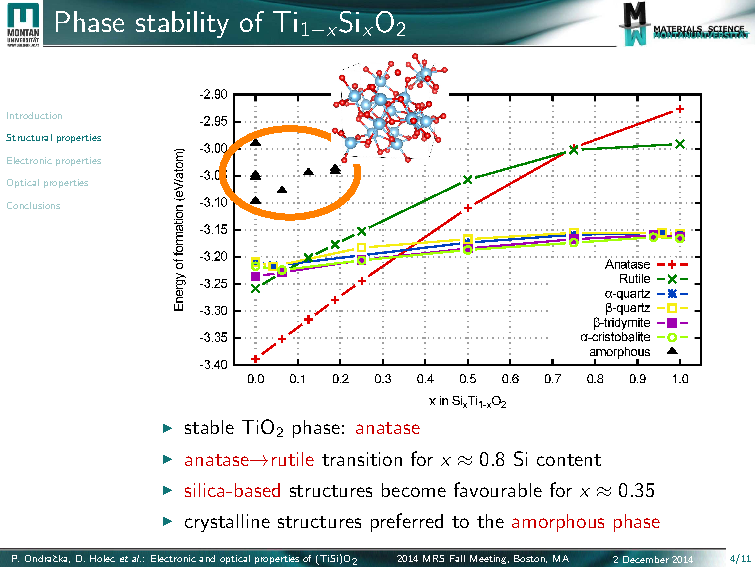
\includegraphics[width=\linewidth]{figures/stability.pdf}
\end{frame}

\section{Problems with amorphous cell generation}
\begin{frame}
    \frametitle{Problems with cell relaxation}
	\begin{columns}
	\begin{column}{0.4\linewidth}
		\begin{itemize}
			\item Simulated annealing process produces cells with residual forces 
			\item This sometimes affects cell properties (like a band gap)
			\item Different relaxation procedures have slightly different results
		\end{itemize}
	\end{column}
	\begin{column}{0.6\linewidth}
		\includegraphics[width=\linewidth]{figures/gap.pdf}
	\end{column}
	\end{columns}

\end{frame}

\begin{frame}
    \frametitle{Relaxation changes in amorphous cells}
	\begin{columns}
	\begin{column}{0.5\linewidth}
		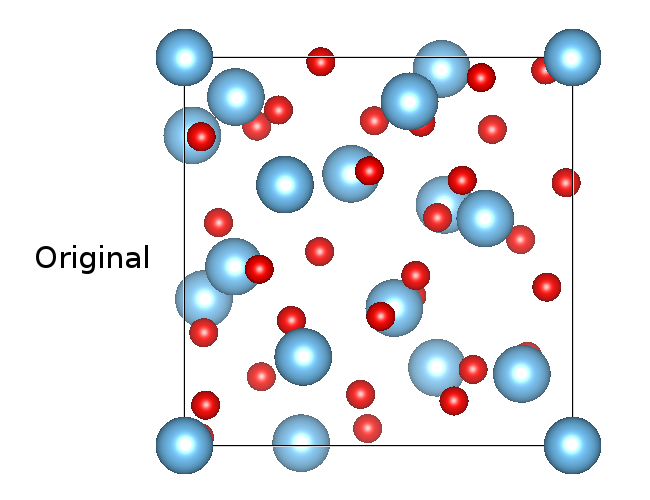
\includegraphics[width=0.9\linewidth]{figures/original.png}
		\newline
		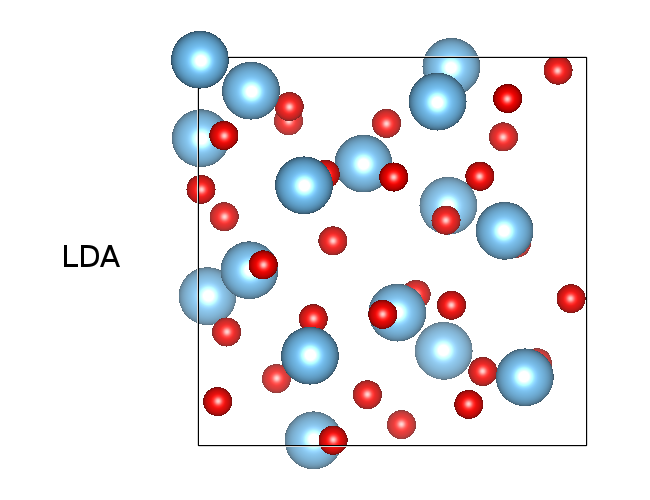
\includegraphics[width=0.9\linewidth]{figures/LDA.png}
	\end{column}
	\begin{column}{0.5\linewidth}
		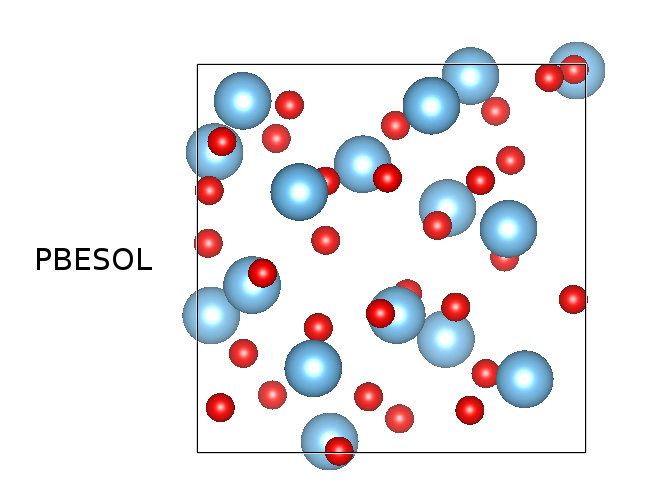
\includegraphics[width=0.9\linewidth]{figures/PBE.png}
		\newline
		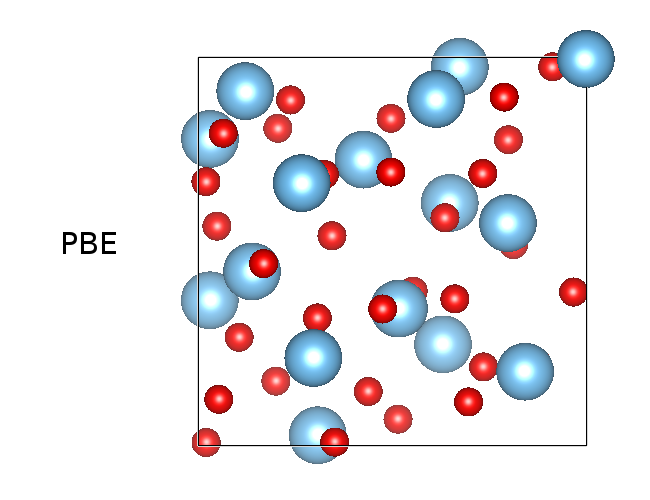
\includegraphics[width=0.9\linewidth]{figures/PBESOL.png}
	\end{column}
	\end{columns}
\end{frame}

\section{Ti$_{1-x}$X$_x$O$_2$ solid solutions}
\begin{frame}
	\includegraphics[width=0.9\linewidth]{figures/gap-overview.pdf}
\end{frame}



\end{document}
